\section{Multiplexer Silicon Results}
\label{sec:multiplexer_silicon_res}
After silicon was received, the worst round trip latency was measured to be \qty{20}{\ns} as shown in Fig~\ref{fig:round_trip_latency_rising_edge} and \ref{fig:round_trip_latency_falling_edge}. Some designs have been validated, including a VGA clock project (Fig.~\ref{fig:VGA_clock_design_TT03_5_silicon}) that takes advantage of the new higher speed IO.

\begin{figure}[!t]
\centering
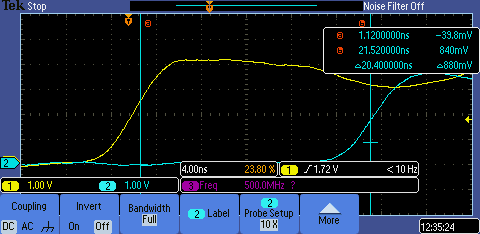
\includegraphics[width=\columnwidth]{./Figs/tt3p5 rising latency.PNG}
\caption{Round trip latency on a rising edge of about \qty{20}{\ns}.}
\label{fig:round_trip_latency_rising_edge}
\end{figure}

\begin{figure}[!t]
\centering
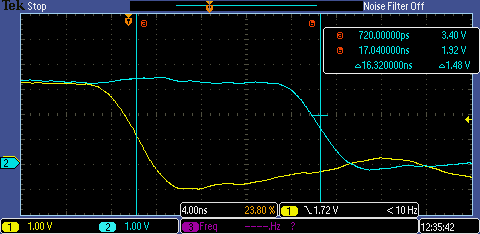
\includegraphics[width=\columnwidth]{./Figs/tt3p5 falling latency.PNG}
\caption{Round trip latency on a falling edge of about \qty{16}{\ns}.}
\label{fig:round_trip_latency_falling_edge}
\end{figure}

\begin{figure}[!t]
\centering
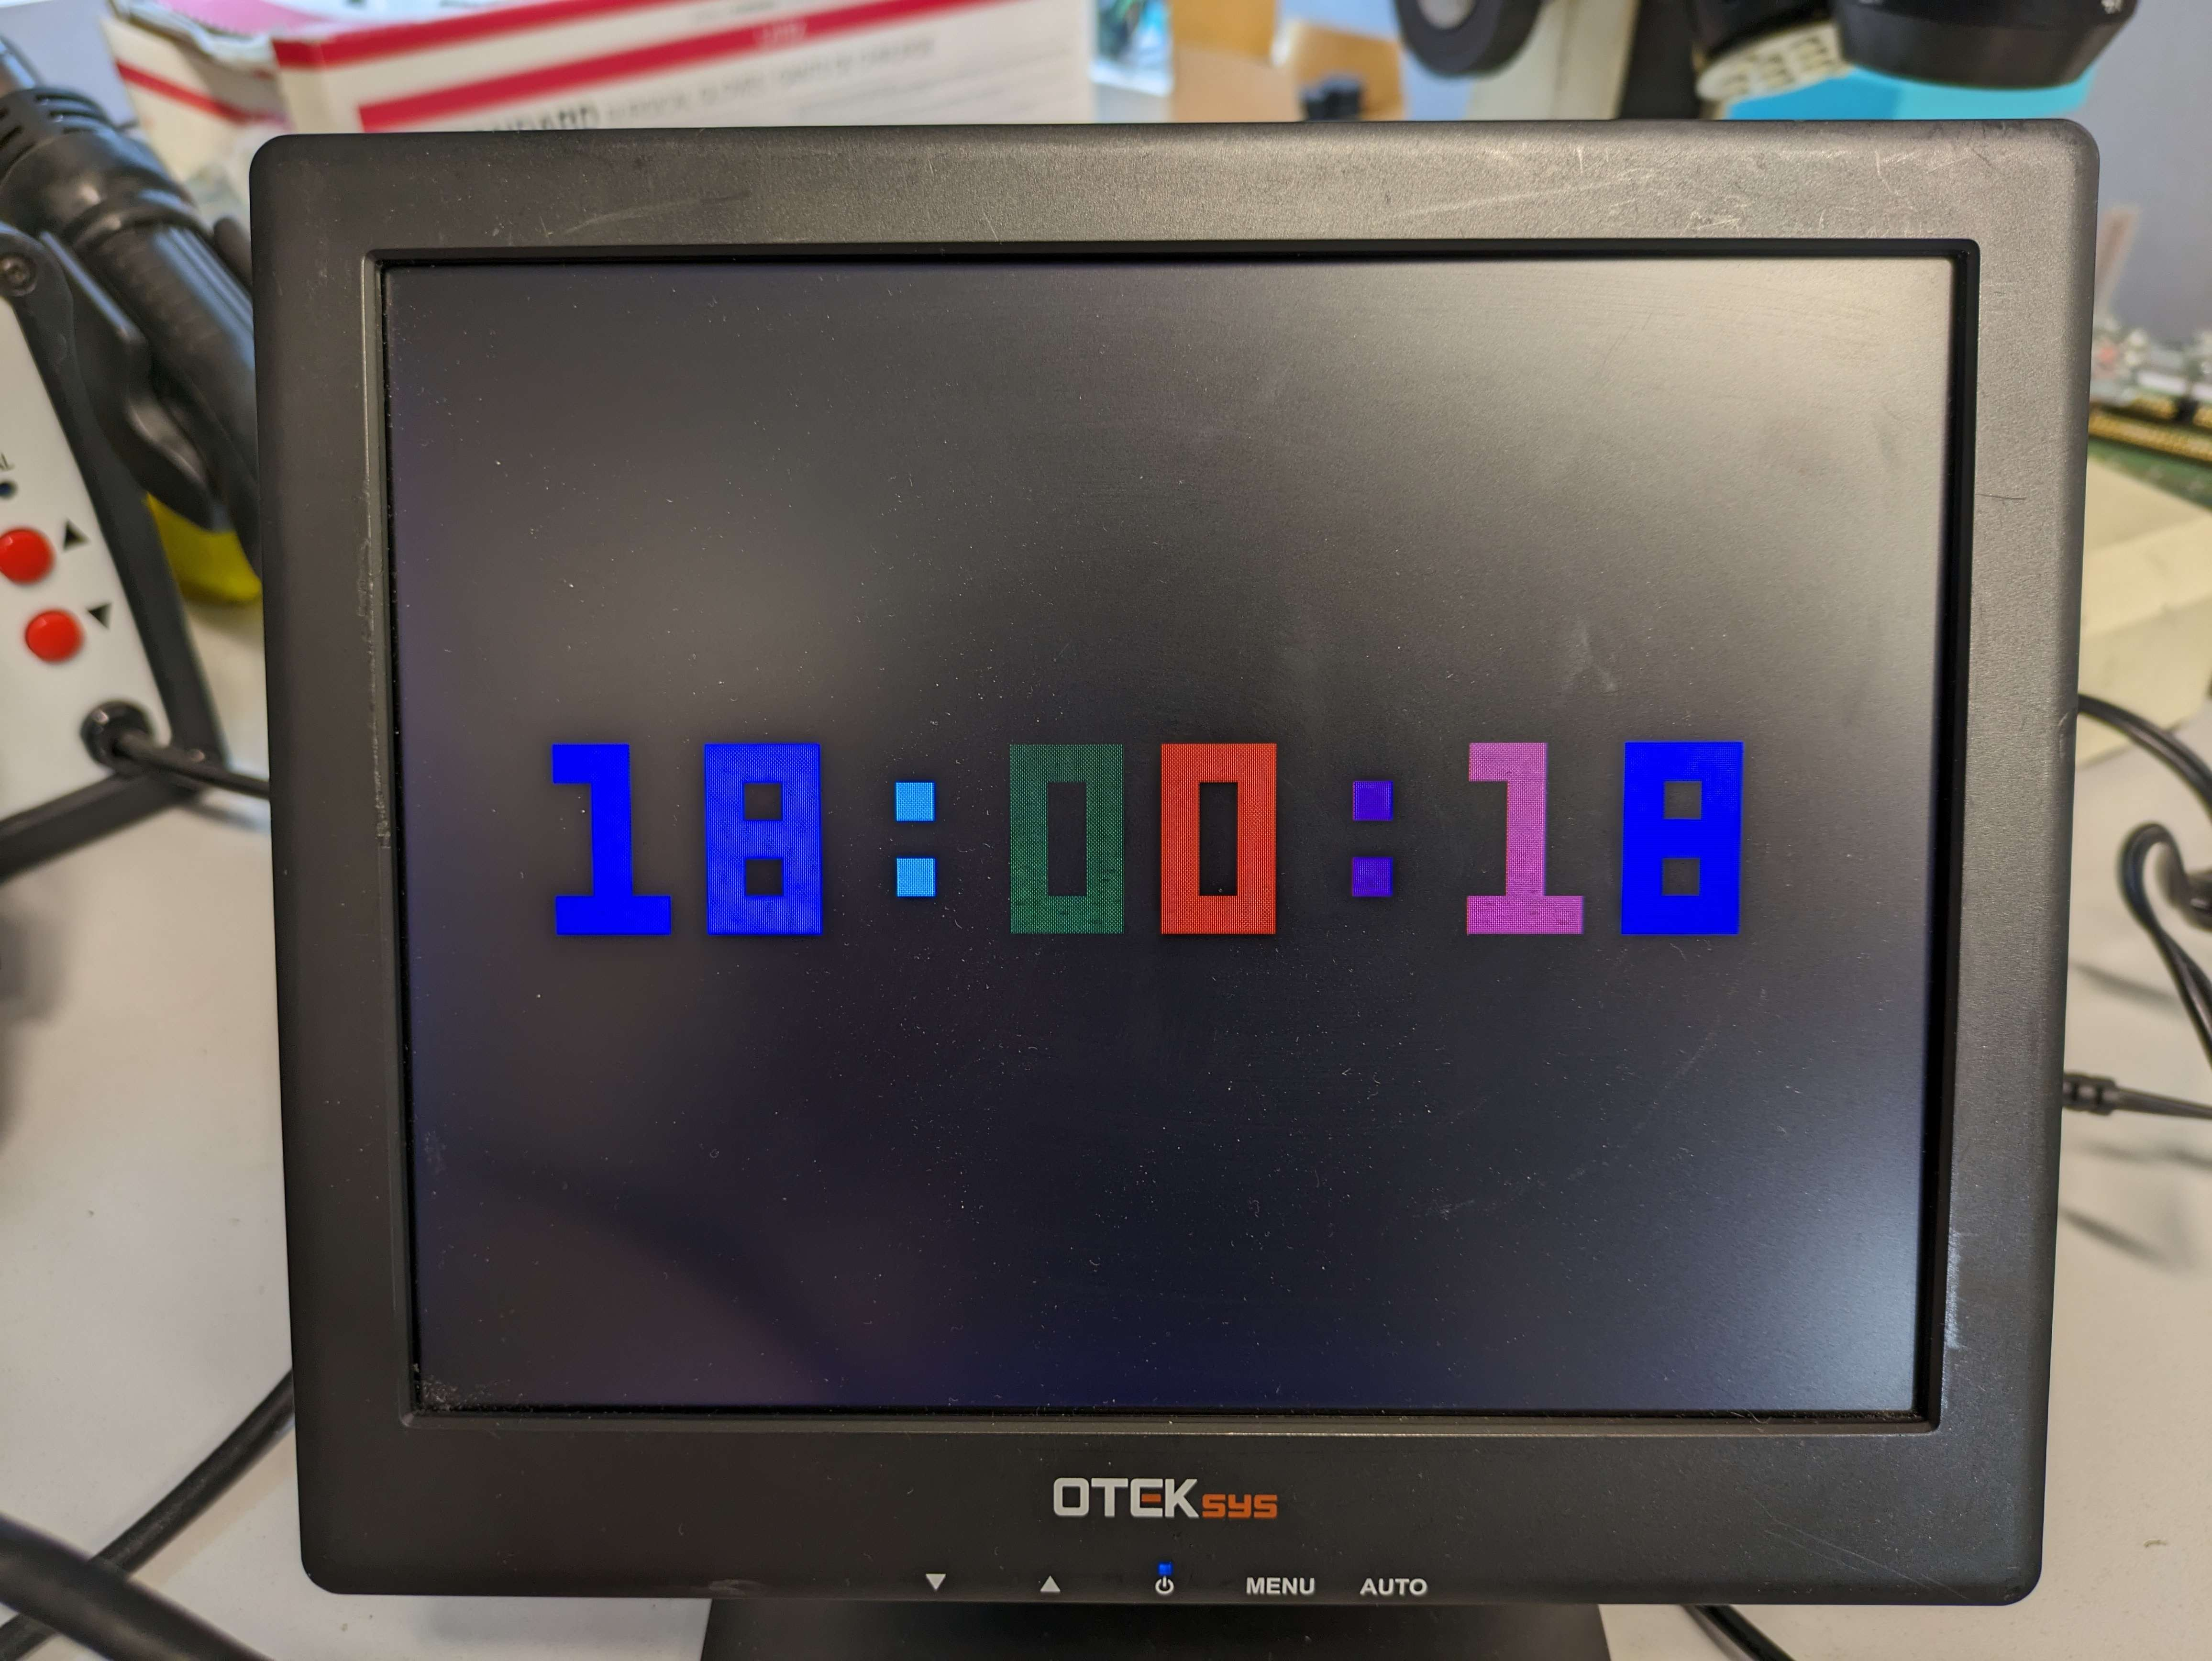
\includegraphics[width=\columnwidth]{./Figs/tt3p5 vga clock.jpg}
\caption{VGA clock design running on TT03.5 silicon.}
\label{fig:VGA_clock_design_TT03_5_silicon}
\end{figure}

The new chip pinout and serial design selection required a new demonstration board (Fig.~\ref{fig:TT04plus_demo_board}) that included an easy way to select the design.
The RP2040 microcontroller was chosen as a co-processor as it allows:

\begin{itemize}
\item Drag and drop firmware updates on any OS,
\item Runs MicroPython\cite{micropython}, ideal for beginners to enable and test their designs (Fig.~\ref{fig:micropython_program}),
\item External memory emulation via PIO and DMA.
\end{itemize}

\begin{figure}[!t]
\centering
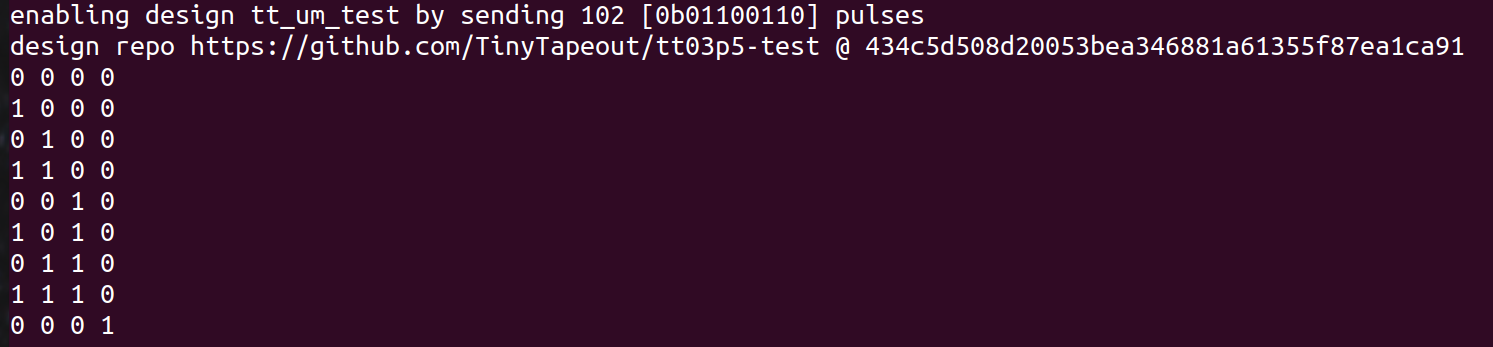
\includegraphics[width=\columnwidth]{./Figs/tt3p5 enable design.png}
\caption{A MicroPython program\cite{demofirmwaretest} enabling a design, clocking it, and printing the results.}
\label{fig:micropython_program}
\end{figure}

\begin{figure}[!t]
\centering
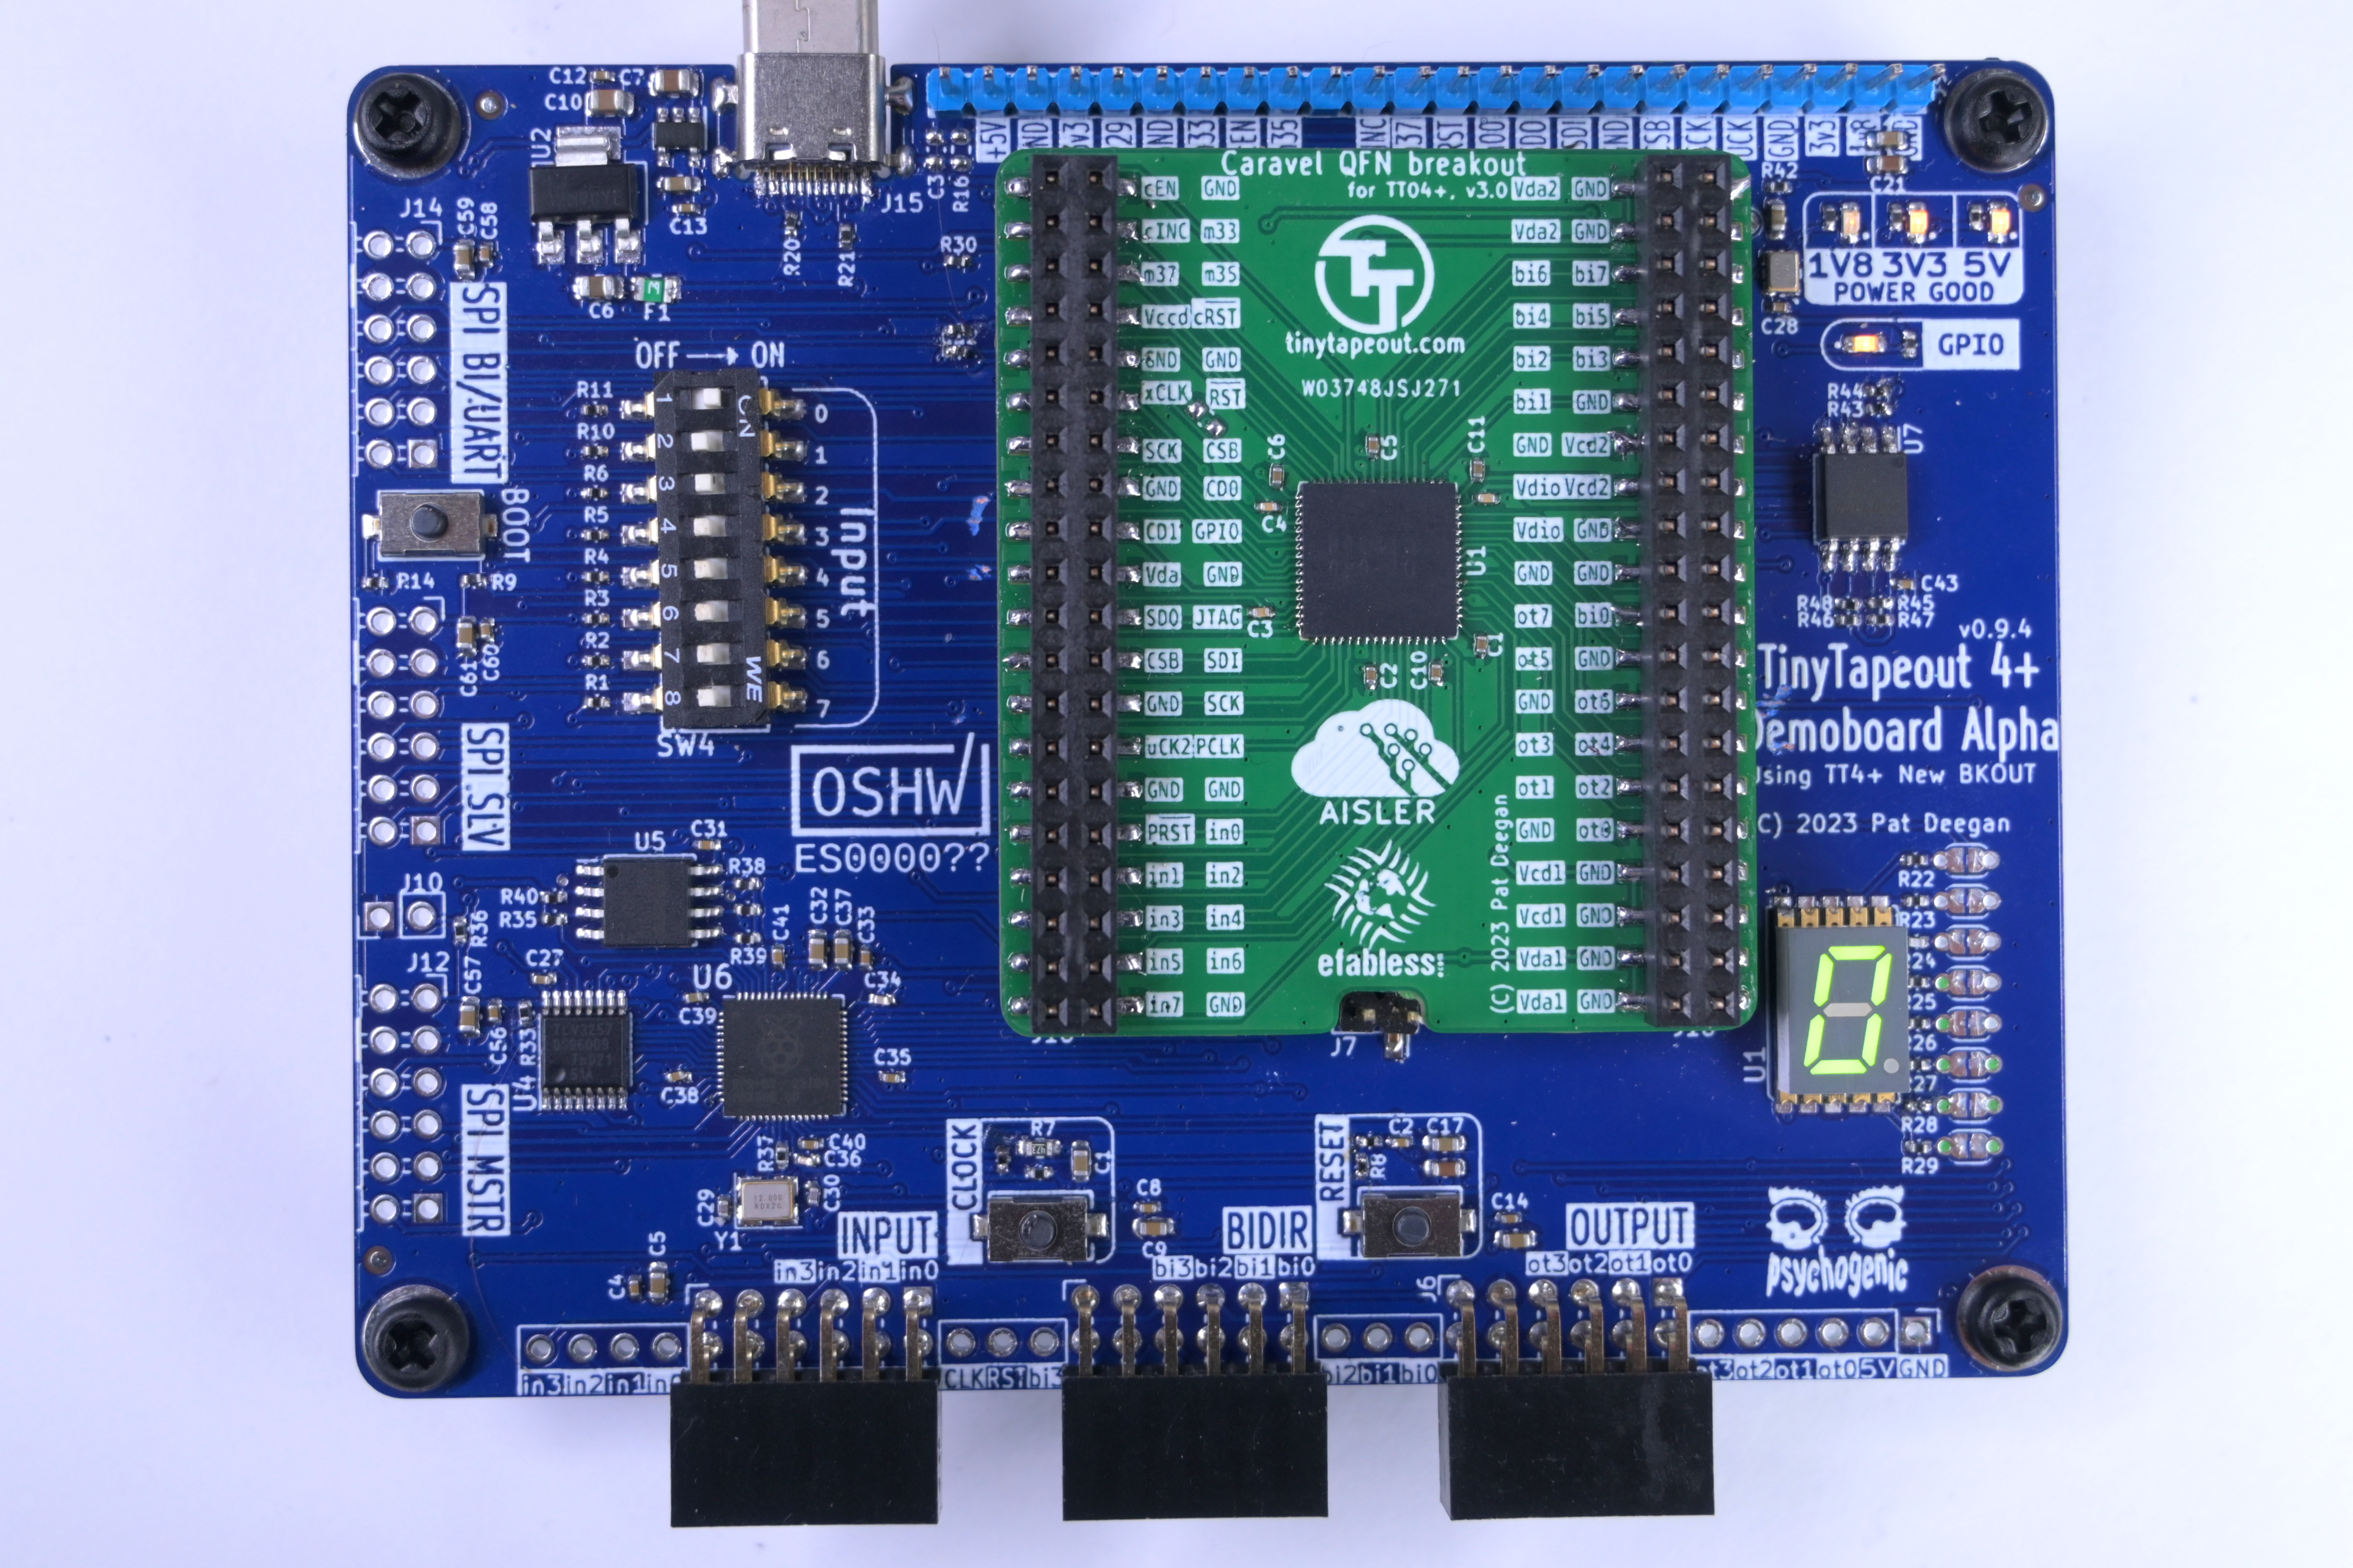
\includegraphics[width=\columnwidth]{./Figs/tt04-demoboard-top.jpg}
\caption{The TT04+ demo board\cite{tt04demoboard}.}
\label{fig:TT04plus_demo_board}
\end{figure}

An additional PMOD expansion port was added for the bidirectional pins, and the community has started to standardize on pinouts~\cite{pinouts} making it easier to test each other's designs.
A new repository was created to house user-contributed PMODs~\cite{awesomepmods}, for example the VGA PMOD shown in Fig.~\ref{fig:user_contributed_VGA_PMOD}.

An additional set of 3 PMOD expansion ports were added that mixed input and outputs, allowing the most common standard PMODs to be used. For more information about the circuit board, pinout and PMOD support see the repository~\cite{tt04demoboard}.

\begin{figure}[!t]
\centering
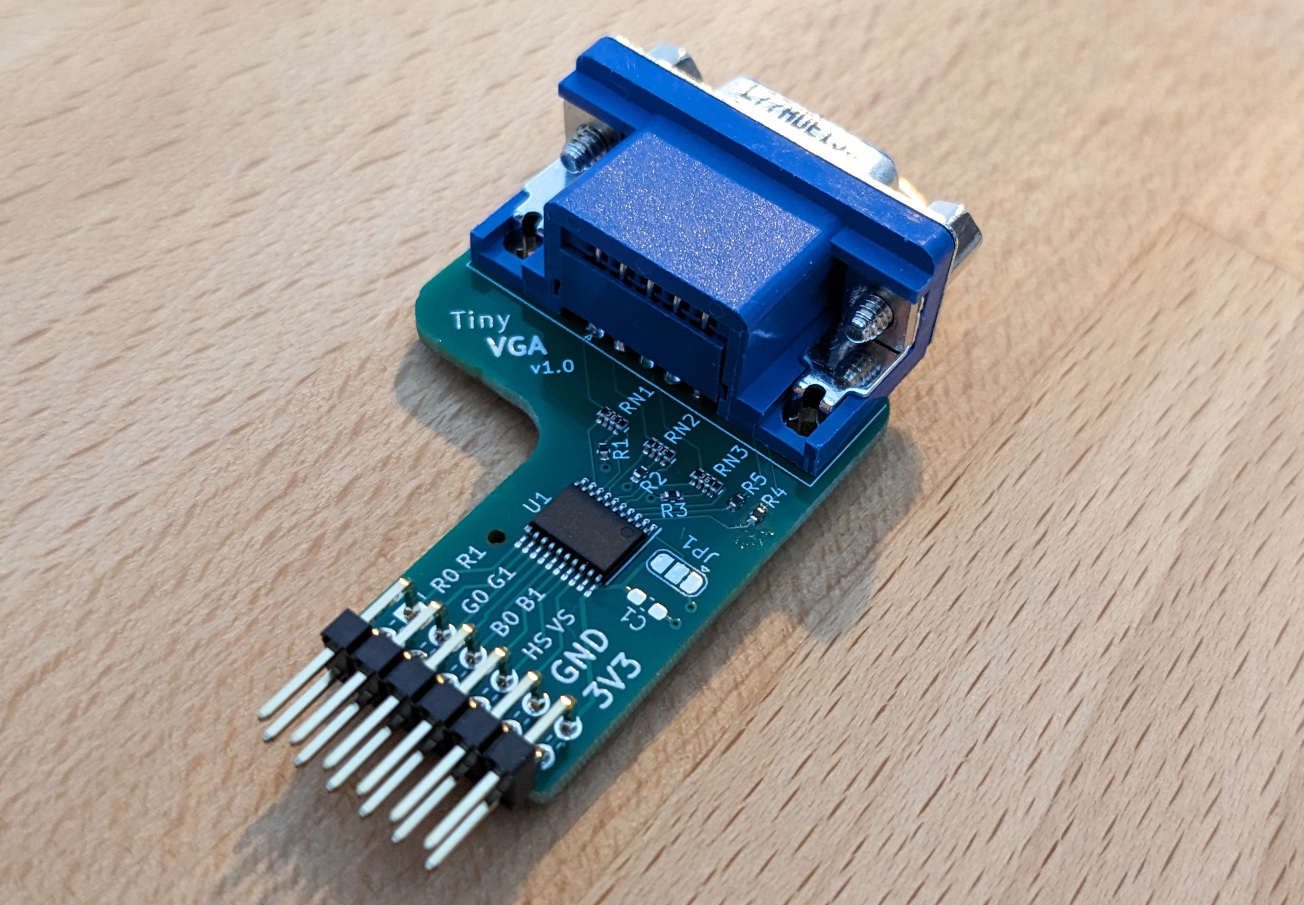
\includegraphics[width=\columnwidth]{./Figs/tiny_vga_pmod.jpg}
\caption{A user-contributed VGA output PMOD.}
\label{fig:user_contributed_VGA_PMOD}
\end{figure}

